\documentclass[../report.tex]{subfiles}


\begin{document}


\section{Introduction}
\label{introduction}

\subsection{What problem does the project focus on?}
\label{What problem does the project focus on?}

This project focuses on the problem of creating the best reinforcement learning agent for a custom made Reversi enviroment.
Reversi is a checkers-like peice capturing board game where peices are placed adjacent to existing opponent board peices, capturing all opponent peices between the new peice and the nearest ally peice.
Here is a simple example of a couple moves in Reversi.
\begin{figure}[h]
    %\fbox{\rule[-.5cm]{0cm}{4cm} \rule[-.5cm]{10cm}{0cm}}
    \centering
    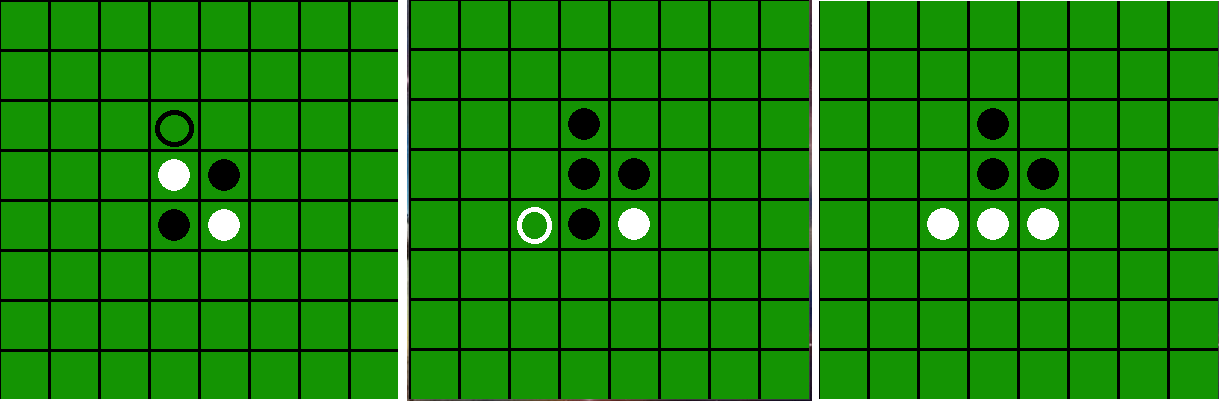
\includegraphics[width=10cm]{ReversiMoves}
    \caption{Two simple starting moves in Reversi}
\end{figure}
The game of reversi ends when the neither player can make a legal move, which typically means the game board is filled.
Once the game has ended, the scoring is simple. The winner of Reversi is the player with the most game peices on the board at the end of the game.

This problem is made complex by the $8\times8$ sized board which contains approximately $3^{64}$ possible states, 
each with an set of actions $\geq0$.

With such a state and action space, tabular solutions are not practical, which makes different function approximation and Deep RL solutions attractive.
Since there are multiple methods to approach this problem, our project implements multiple algorithms and compares them against a baseline (Random) player.


\subsection{Why should we care about this problem?}
\label{Why should we care about this problem?}
    some text

\end{document}